

%\documentclass{book}\begin{document}<content\end{document}
\documentclass[letter, 11pt, margins=0.25in]{texMemo}  % The texMemo package by Rob Oakes.

\usepackage{amsmath}
\usepackage{color, soul}
\usepackage[colorlinks=true, citecolor=blue]{hyperref}
\usepackage{enumitem}
\usepackage{graphicx, lipsum}

\usepackage[LGRgreek]{mathastext}

\usepackage{matlab-prettifier}
\usepackage{multirow}

\usepackage{natbib}
\bibliographystyle{apalike}

\usepackage[table]{xcolor}
\definecolor{maroon}{cmyk}{0,0.87,0.68,0.32}
\definecolor{LightCyan}{rgb}{0.88,1,1}
\definecolor{Gray}{gray}{0.85}


\memodate{\today~(Submitted)}
%\memoto{Dr. Dan Russell - College of Engineering, Penn State University}
%\memofrom{Michael R. Wirtzfeld - Sound Discovery LLC\\}
\memosubject{Noise Control Applications - Module 1 Assignement\\}

%\memologo{
\includegraphics[width=1.0\textwidth]{SOUND_DISCOVERY_Business_Card.jpg}}



\begin{document}

\maketitle


\vspace{-0.25cm}
\section*{Problem 1 - Cut-on Frequencies in Ducts and Pipes}

The Matlab code for this problem is listed in Appendix~\ref{appendix:problem1}.

\vspace{-0.25cm}
\subsection*{Problem 1a}

The lowest cut-on frequency for a rectangular duct with air flow is given by equation,

\vspace{-0.25cm}
\begin{equation}
    f_{cut-on} = 0.5 \cdot \frac{c}{L}
\end{equation}

where $c$ is the speed of sound in air, 343~$\frac{m}{s}$,  and $L$ is the largest side of the rectangular cross-section.

\vspace{0.25cm}
With cross-sectional dimensions of $L_x = 12~cm$ and $L_y = 20~cm$, the lowest cut-on frequency for this rectangular duct is,

\vspace{-0.25cm}
\begin{equation*}
    f_{cut-on} = 0.5 \cdot \frac{ 343~\frac{m}{s} }{ 0.20~m } = \boldsymbol{857.5~Hz}
\end{equation*}



\vspace{-0.25cm}
\subsection*{Problem 1b}

The lowest cut-on frequency for a circular duct with air flow with the same cross-sectional area as the rectangular duct in part (a.) can be calculated using equation,

\vspace{-0.25cm}
\begin{equation}
    f_{cut-on} = 0.568 \cdot \frac{c}{d}
    \label{equation:circularDuct}
\end{equation}

where $c$ is the speed of sound in air, 343~$\frac{m}{s}$,  and $d$ is diameter of the circular duct.

\vspace{0.25cm}
The cross-sectional area of the rectangular duct is,

\vspace{-0.25cm}
\begin{equation*}
    Area_{~rectangular~duct} = 0.12~m~\cdot0.20~m =  0.024~m
\end{equation*}

\vspace{0.25cm}
The corresponding diameter for this area is,

\vspace{-0.25cm}
\begin{equation*}
    diameter = \sqrt{ \frac{0.24~m^2}{\pi} } \cdot 2 = 0.17~m
\end{equation*}

\vspace{0.25cm}
Using Eq.~\ref{equation:circularDuct}, the lowest cut-on frequency for this circular duct with air flow is,

\vspace{-0.25cm}
\begin{equation*}
    f_{cut-on} = 0.568 \cdot \frac{ 1,500~\frac{m}{s} }{ 0.17~m } = \boldsymbol{1,114.5~Hz}
\end{equation*}




\vspace{-0.25cm}
\subsection*{Problem 1c}

The lowest cut-on frequency for this circular duct with water flow can be calculated using Eq.~\ref{equation:circularDuct},

\vspace{-0.25cm}
\begin{equation*}
    f_{cut-on} = 0.568 \cdot \frac{ 1,500~\frac{m}{s} }{ 0.17~m } = \boldsymbol{4,873.9~Hz}
\end{equation*}

The lowest cut-on frequency for water is considerable larger than it is for air flow.





\vspace{-0.25cm}
\subsection*{Problem 1d}

The speed of sound in air is calculated by,

\vspace{-0.25cm}
\begin{equation}
    c = \sqrt{ \gamma \cdot R \cdot T_K }
    \label{equation:speedOfSoundInAir}
\end{equation}

where $\gamma = 1.4$ is the ratio of specific heats, $R = 287~\frac{J}{kg \cdot K}$ is the gas constant, and $T_K$ is the absolute temperature in Kelvin.

\vspace{0.25cm}
Figure~\ref{figure:cuton_frequency_versus_temperature} illustrates how the lowest cut-on frequency changes as the air heats from $0^{\circ}$ to $500^{\circ}$ Celsius.

\vspace{0.25cm}
The square-root relationship between temperature and the speed of sound in air is apparent and governs the behaviour of the cut-on frequency.




\vspace{-4.8cm}
\begin{figure}[!htb]

    \center
        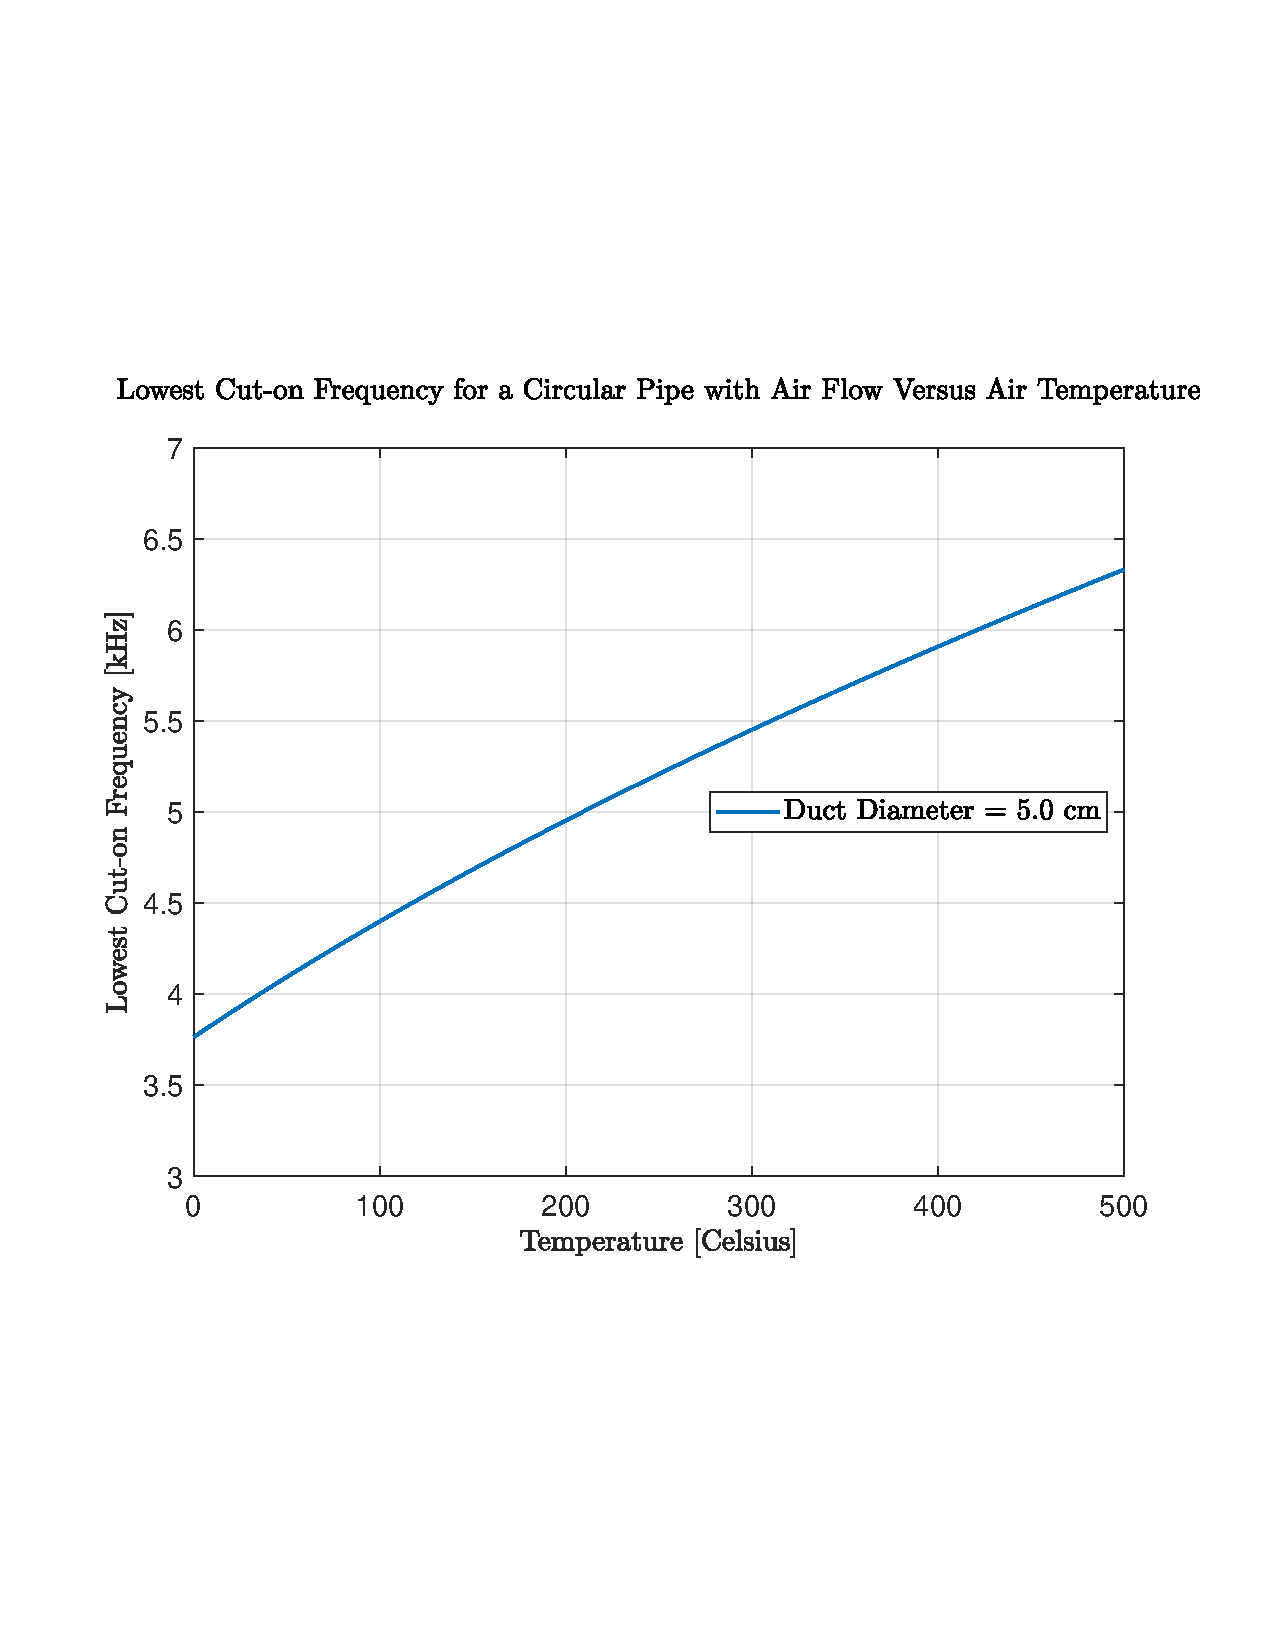
\includegraphics[ scale = 0.8, keepaspectratio ]{Cut-on Frequency Versus Temperature - Sunday, January 19, 2025.pdf}

    \vspace{-5.2cm}
    \caption{Lowest cut-on frequency for a circular 5 cm diameter duct versus air temperature.}
    \label{figure:cuton_frequency_versus_temperature}

\end{figure}





\vspace{-0.25cm}
\subsection*{Problem 1e}

 \textbf{Question:  Are cut-on frequencies higher for a circular or rectangular duct for a given cross-sectional area?}

 The lowest cut-on frequency is higher for a circular duct than for a
 rectangular duct for a given cross-sectional area.

 For the dimensions given in class, the rectangular duct is not square.
 This produces a larger dimension and thus a smaller, lowest cut-on
 frequency.  If the rectangular duct is square dimensions on the order
 of the circular duct diameter with the same cross-sectional area, the
 cut-on frequencies are approximately equal.



\vspace{0.25cm}
\textbf{Question:  What about in air versus water?}

 The lowest cut-on frequency is larger for water than for air.  The cut-on
 frequency is proportional to the speed of sound and the speed of sound in
 water is greater than the speed of sound in air.



\vspace{0.25cm}
\textbf{Question:  What about cold versus hot air?}

 The lowest cut-on frequency is higher for warm air than it is for cold air.









\newpage
\section*{Problem 2 - Muffler Design Comparison}

The Matlab code for this problem is listed in Appendix~\ref{appendix:problem2}.

For these muffler comparisons, the following assumptions were made:

\begin{itemize}
  \item There is no flow.
  \item There are no resistive terms.
  \item The load impedance was not included because the transmission loss does not require them.
  \item For Parts b, c, and d, the side branch length offset, $L_o$, was set to zero.
\end{itemize}


\vspace{-0.25cm}
\subsection*{Problems 2a, 2b, and 2c}

\vspace{-0.25cm}
Figure~\ref{figure:problem2figure1} shows the transmission loss profiles for a simple expansion chamber, a double-tuned expansion chamber, and a cascaded double-tuned expansion chamber muffler.

The peaks for the simple expansion chamber (red, dashed line) are approximately 22 dB and occur at frequencies with a wavelength that is a quarter of the length of the expansion chamber.  Minimal loss occurs at half wavelength multiples.

The addition of the extension tube inside the muffler produces a quarter wavelength resonator.  The side branch of Ji (2005;  Slide 11, Lecture 3 notes) was used to calculate $L_o$.  For the cascaded double-tuned expansion chamber, the extension tubes produce a secondary quarter wavelength resonator.

As noted in the office hours session, there is no damping which produces artificially high resonances.


\begin{figure}[!htb]

    \center
        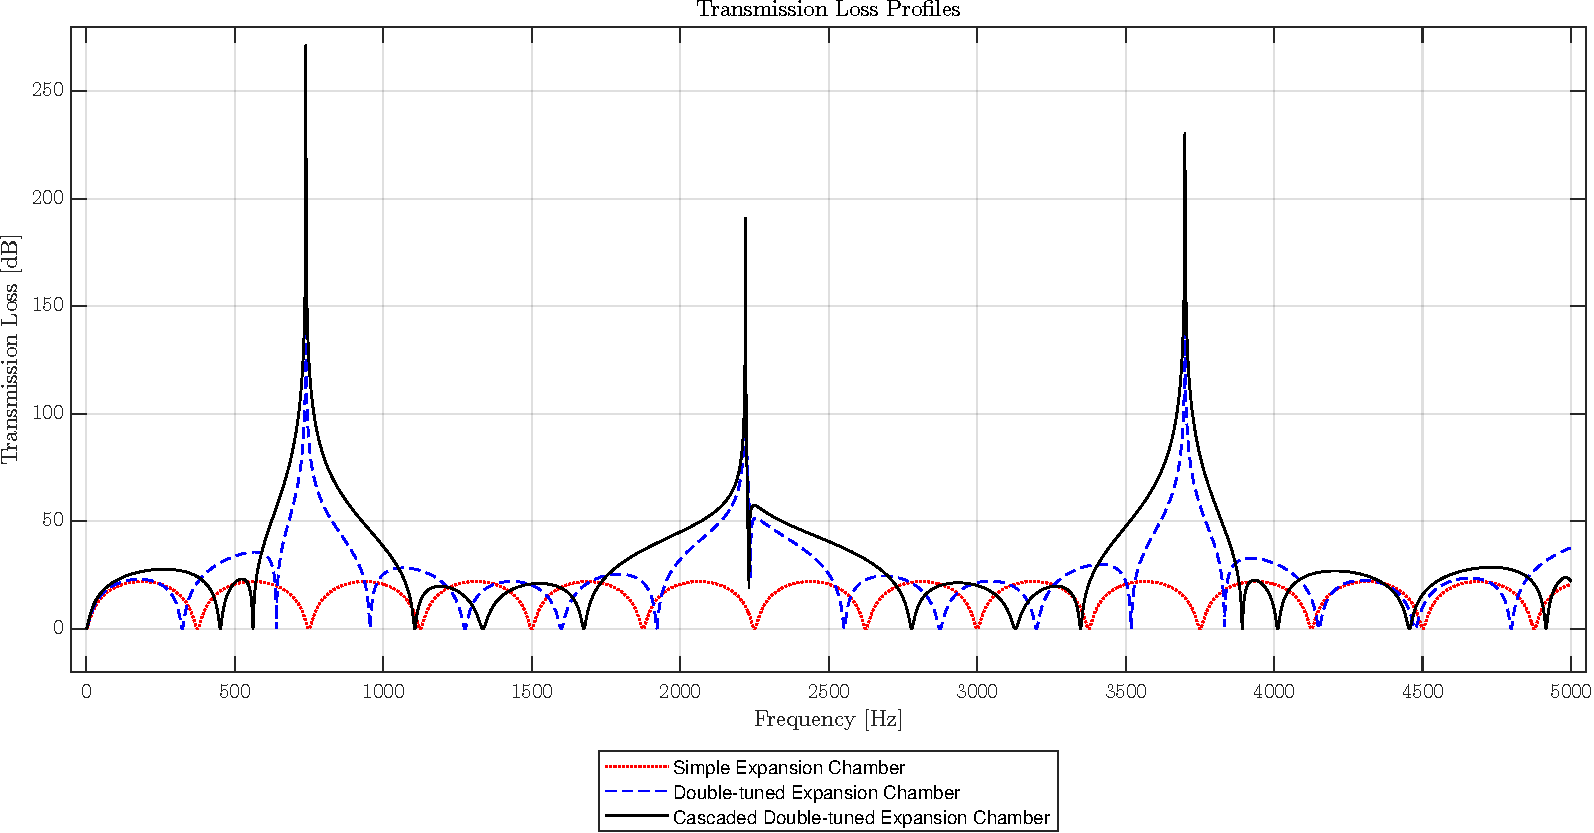
\includegraphics[ scale = 0.675, keepaspectratio ]{Assignment 1 - Question 2 Figure All TL Profiles.pdf}

    \caption{Transmission loss profiles for a simple expansion chamber, a double-tuned expansion chamber, and a cascaded double-tuned expansion chamber mufflers.}
    \label{figure:problem2figure1}

\end{figure}



\subsection*{Problem 2d}

Figure~\ref{figure:problem2figure2} shows the transmission loss profiles for a cascaded double-tuned expansion chamber, and a modified cascaded double-tuned expansion chamber muffler.

Two modifications were made to the original system:

\begin{enumerate}
  \item The left 3" extension tube in the left chamber was shortened to 2" inches, making the respective muffler section 1" longer.
  \item The left 3" extension tube in the right chamber was lengthened to 4", making the respective muffler section 1" shorter.
\end{enumerate}

\vspace{0.5cm}
\begin{figure}[!htb]

    \center
        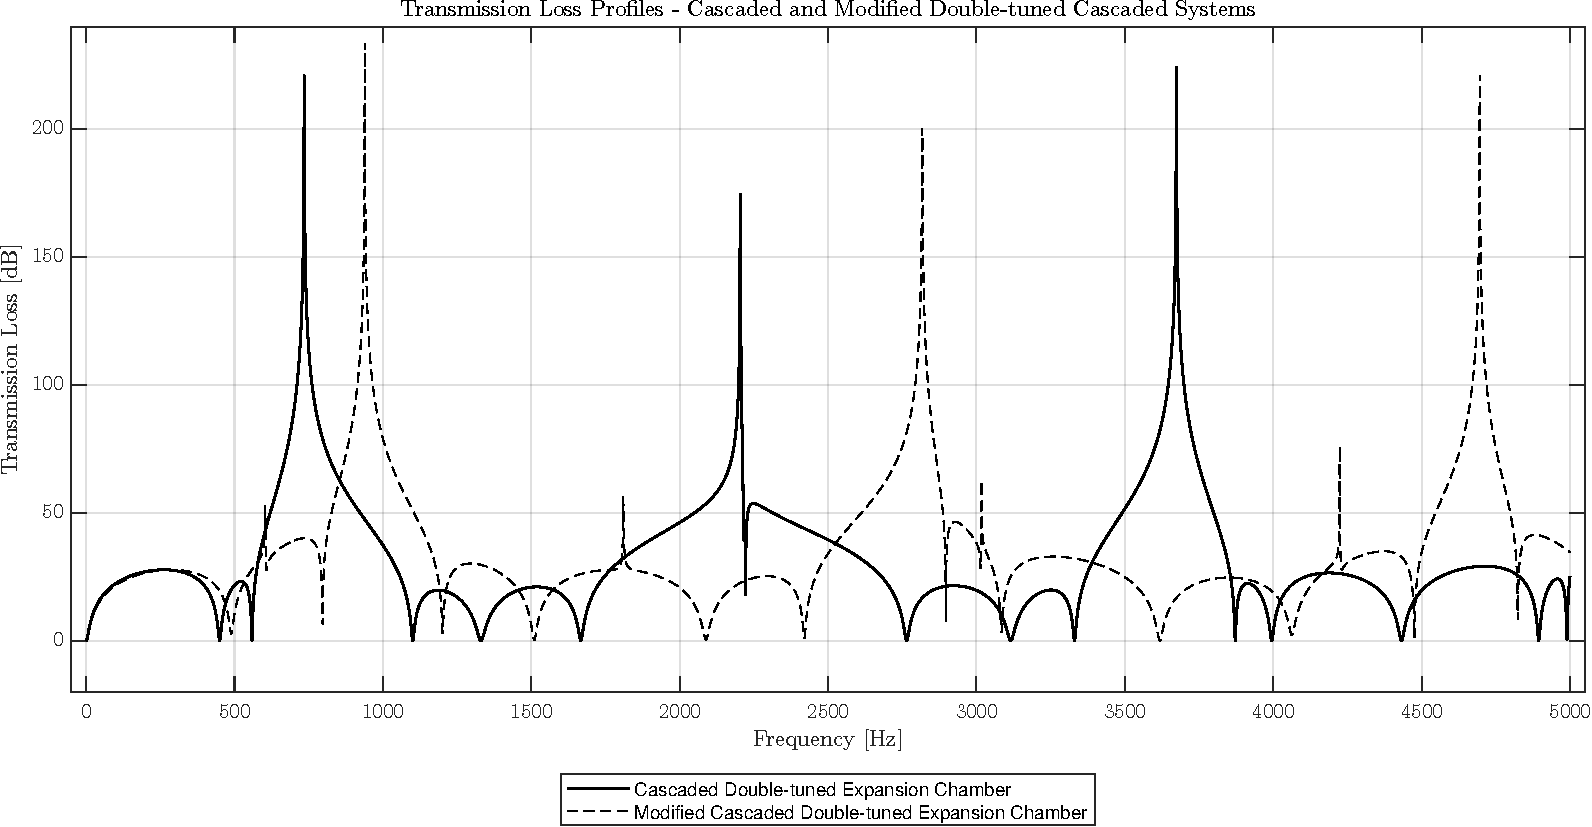
\includegraphics[ scale = 0.675, keepaspectratio ]{Assignment 1 - Question 2 Figure Comparison TL Plot For Cascaded Systems.pdf}

    \caption{Transmission loss profiles for a cascaded double-tuned expansion chamber muffler and a modified version of this muffler.}
    \label{figure:problem2figure2}

\end{figure}

\vspace{0.25cm}
These modifications change the symmetry of the cascaded system, and allow the resonate frequencies to be independently changed.












\newpage
\section*{Problem 3 - Bugle Recorder}


\vspace{-0.25cm}
\subsection*{Problem 3a}

The Matlab code for this problem is listed in Appendix~\ref{appendix:problem3}.

Table~\ref{table:mouthpieceAndPip} lists the length of the pipe section and the mouthpiece.

\setlength{\abovecaptionskip}{0pt}
\vspace{0.1cm}
{\renewcommand{\arraystretch}{1.5}
\begin{table}[h!]
    \begin{center}
        \small
        \begin{tabular}{ | c | c | }
            \hline
            \textbf{Item}  &  \textbf{Length [mm]}  \\
            \hline
                Pipe  &  145  \\
                \hline
                \rowcolor{Gray}
                Mouthpiece  &  90  \\
            \hline
        \end{tabular}
    \end{center}
    \caption{Determined length of the pipe and length of the mouthpiece.}
    \label{table:mouthpieceAndPip}
\end{table}


\vspace{-0.25cm}
\subsection*{Problem 3b}

Table~\ref{table:holePlacementSummary} summarizes the placement of the holes for each note relative to the end of the pipe.

\setlength{\abovecaptionskip}{0pt}
\vspace{0.1cm}
{\renewcommand{\arraystretch}{1.5}
\begin{table}[h!]
    \begin{center}
        \small
        \begin{tabular}{ | c | c | c | }
            \hline
            \textbf{Note}  &  \textbf{Frequency [Hz]}  &  \textbf{Distance from End of Pipe [mm]}  \\
            \hline
                C5  &  523      &  n/a  \\
                \rowcolor{Gray}
                F5  &  698      &  87.8  \\
                A5  &  880      &  0  \\
                \rowcolor{Gray}
                C6  &  1,046    &  0  \\
            \hline
        \end{tabular}
    \end{center}
    \caption{Hole placement distances.}
    \label{table:holePlacementSummary}
\end{table}


\vspace{-0.25cm}
\subsection*{Problem 3 - Comments}

Diameters of holes should be smaller than a wavelength.

Issue with impedance.










\newpage
\section*{Problem 4 - Intake Duct}

\subsection*{Problem 4a}

\subsection*{Problem 4b}

\subsection*{Problem 4c}

\subsection*{Problem 4d}










\newpage
\section*{Problem 5 - Intake Duct Silencer}

\subsection*{Problem 5a}

\subsection*{Problem 5b}

\subsection*{Problem 5c}

\subsection*{Problem 5d}

\subsection*{Problem 5e}






\newpage
\section{Appendix - Matlab Code for Problem 1}
\label{appendix:problem1}

\lstinputlisting[style=Matlab-Pyglike, basicstyle=\fontfamily{pcr}, numbers=left, keepspaces, mlshowsectionrules, basicstyle=\scriptsize]{../ACS_597_Module_1_Question_1_Monday_January_13_2025.m}



\newpage
\section{Appendix - Matlab Code for Problem 2}
\label{appendix:problem2}

\lstinputlisting[style=Matlab-Pyglike, basicstyle=\fontfamily{pcr}, numbers=left, keepspaces, mlshowsectionrules, basicstyle=\scriptsize]{../ACS_547_Module_1_Question_2_Monday_January_27_2025.m}



\newpage
\section{Appendix - Matlab Code for Problem 3}
\label{appendix:problem3}

\lstinputlisting[style=Matlab-Pyglike, basicstyle=\fontfamily{pcr}, numbers=left, keepspaces, mlshowsectionrules, basicstyle=\scriptsize]{../ACS_547_Module_1_Question_3_Wednesday_January_29_2025.m}



\newpage
\section{Appendix - Matlab Code for Problem 4}
\label{appendix:problem4}

\lstinputlisting[style=Matlab-Pyglike, basicstyle=\fontfamily{pcr}, numbers=left, keepspaces, mlshowsectionrules, basicstyle=\scriptsize]{../ACS_547_Module_1_Question_4_Wednesday_January_29_2025.m}



\newpage
\section{Appendix - Matlab Code for Problem 5}
\label{appendix:problem5}

\lstinputlisting[style=Matlab-Pyglike, basicstyle=\fontfamily{pcr}, numbers=left, keepspaces, mlshowsectionrules, basicstyle=\scriptsize]{../ACS_547_Module_1_Question_5_Friday_January_31_2025.m}







\end{document}






% Reference(s):

% https://tex.stackexchange.com/questions/180222/how-to-change-font-size-for-specific-lstlisting


































